\documentclass[border=10pt]{standalone}

\usepackage[utf8]{inputenc}
\usepackage[english]{babel}
\usepackage{tikz}
\usetikzlibrary{positioning, arrows.meta, fit}

\begin{document}
	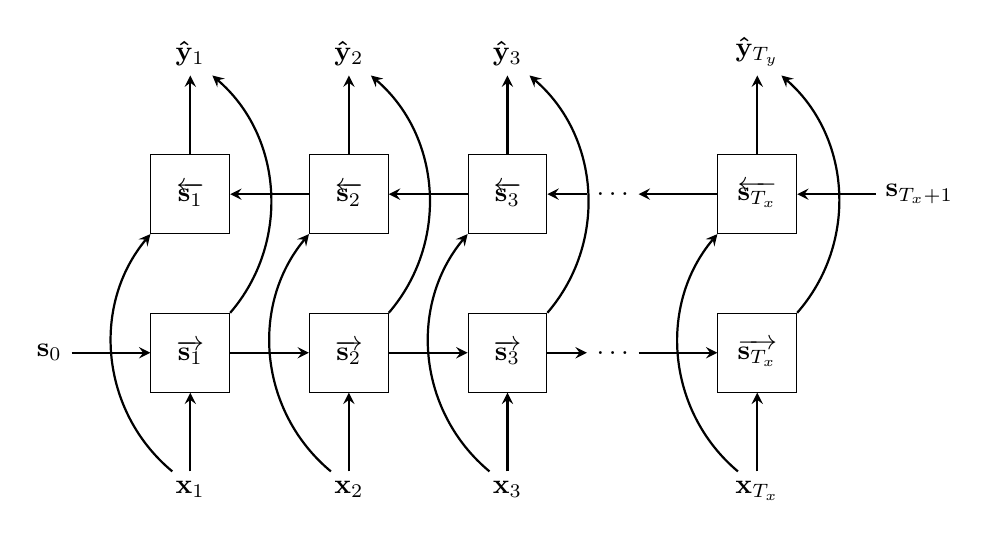
\begin{tikzpicture}
		% forward rnn
		\node[rectangle, draw, minimum height=1cm, minimum width=1cm] (ar1) {$\overrightarrow{\mathbf{s}_{1}}$};
		\node[rectangle, right=of ar1, draw, minimum height=1cm, minimum width=1cm] (ar2) {$\overrightarrow{\mathbf{s}_{2}}$};
		\node[rectangle, right=of ar2, draw, minimum height=1cm, minimum width=1cm] (ar3) {$\overrightarrow{\mathbf{s}_{3}}$};
		\node[rectangle, right=0.5 of ar3] (ar5) {$\dots$};
		\node[rectangle, right= of ar5, draw, minimum height=1cm, minimum width=1cm] (artx) {$\overrightarrow{\mathbf{s}_{T_{x}}}$};
		\node[left=of ar1] (ar0) {$\mathbf{s}_{0}$};
		% backwards rnn
		\node[rectangle, above=of ar1, draw, minimum height=1cm, minimum width=1cm] (al1) {$\overleftarrow{\mathbf{s}_{1}}$};
		\node[rectangle, right=of al1, minimum height=1cm, minimum width=1cm, draw] (al2) {$\overleftarrow{\mathbf{s}_{2}}$};
		\node[rectangle, right=of al2, minimum height=1cm, minimum width=1cm, draw] (al3) {$\overleftarrow{\mathbf{s}_{3}}$};
		\node[rectangle, right=0.5 of al3] (al5) {$\dots$};
		\node[rectangle, right= of al5, draw, minimum height=1cm, minimum width=1cm] (altx) {$\overleftarrow{\mathbf{s}_{T_{x}}}$};
		\node[right=of altx] (altx1) {$\mathbf{s}_{T_{x}+1}$};
		% inputs	
		\node[below=of ar1] (X1) {$\mathbf{x}_{1}$};
		\node[below=of ar2] (X2) {$\mathbf{x}_{2}$};
		\node[below=of ar3] (X3) {$\mathbf{x}_{3}$};
		\node[below=of artx] (Xt) {$\mathbf{x}_{T_{x}}$};	
		% outputs 
		\node[above=of al1] (Y1) {$\mathbf{\hat{y}}_{1}$};
		\node[above=of al2] (Y2) {$\mathbf{\hat{y}}_{2}$};
		\node[above=of al3] (Y3) {$\mathbf{\hat{y}}_{3}$};
		\node[above=of altx] (Yt) {$\mathbf{\hat{y}}_{T_{y}}$};
		% forward input arrows	
		\draw[-stealth, thick] (X1) -- (ar1);
		\draw[-stealth, thick] (X2) -- (ar2);
		\draw[-stealth, thick] (X3) -- (ar3);
		\draw[-stealth, thick] (Xt) -- (artx);
		% forward hidden states
		\draw[-stealth, thick] (ar1) -- node[above, pos=0.35] {} (ar2);
		\draw[-stealth, thick] (ar2) -- node[above, pos=0.35] {} (ar3);
		\draw[-stealth, thick] (ar3) -- (ar5);
		\draw[-stealth, thick] (ar5) -- (artx);
		\draw[-stealth, thick] (ar0) -- (ar1);
		% backwards hidden states
		\draw[-stealth, thick] (al2) -- node[above, pos=0.35] {} (al1);
		\draw[-stealth, thick] (al3) -- node[above, pos=0.35] {} (al2);
		\draw[-stealth, thick] (al5) -- (al3);
		\draw[-stealth, thick] (altx) -- (al5);
		\draw[-stealth, thick] (altx1) -- (altx);
		% backwards input arrows	
		\path[-stealth, thick] (X1) edge[bend left=45] (al1);
		\path[-stealth, thick] (X2) edge[bend left=45] (al2);
		\path[-stealth, thick] (X3) edge[bend left=45] (al3);
		\path[-stealth, thick] (Xt) edge[bend left=45] (altx);
		% forward output arrows
		\path[-stealth, thick] (ar1) edge[bend right=45] (Y1);
		\path[-stealth, thick] (ar2) edge[bend right=45] (Y2);
		\path[-stealth, thick] (ar3) edge[bend right=45] (Y3);
		\path[-stealth, thick] (artx) edge[bend right=45] (Yt);
		% backwards output arrows	
		\draw[-stealth, thick] (al1) -- (Y1);
		\draw[-stealth, thick] (al2) -- (Y2);
		\draw[-stealth, thick] (al3) -- (Y3);
		\draw[-stealth, thick] (altx) -- (Yt);
	\end{tikzpicture}
\end{document}